\documentclass[11pt]{article}

\usepackage{graphicx}    % needed for including graphics e.g. EPS, PS
\usepackage{pst-sigsys}

 \topmargin -1cm        % read Lamport p.163
 \oddsidemargin -0.04cm   % read Lamport p.163
 \evensidemargin -0.04cm  % same as oddsidemargin but for left-hand pages
 \textwidth 16.59cm
 \textheight 21.94cm 
 %\pagestyle{empty}       % Uncomment if don't want page numbers
 \parskip 7.2pt           % sets spacing between paragraphs
 %\renewcommand{\baselinestretch}{1.5} 	% Uncomment for 1.5 spacing between lines
 \parindent 0pt		  % sets leading space for paragraphs

\newenvironment{mylisting}
{\begin{list}{}{\setlength{\leftmargin}{1em}}\item\scriptsize\bfseries}
{\end{list}}

\newenvironment{mytinylisting}
{\begin{list}{}{\setlength{\leftmargin}{1em}}\item\tiny\bfseries}
{\end{list}}


\title{System Design Document - rev 1.0\\
 Animal Simulation}
\author{Trevor Douglas\\
Software Systems Lab Instructor\\
University of Regina\\
trevor.douglas@uregina.ca\\
Office: ED 473}


 \begin{document}         
 % Start your text
\maketitle

\section{Introduction}
\subsection{Purpose}
The purpose is to create a virtual environment in which these animals live.  No external forces such as weather will affect our system.
\subsection{Design Goals}
The rules laid out shall be:
\begin{itemize}
  \item World is 150 kms square.  Carve up the world into a grid of 150/150 (2D environment)
  \item Animals without wings can travel three kms in a day. (3 grid locations)
  \item Animals with wings can travel 5kms. 
  \item Insects can travel 1km.
  \item Everything must eat within two days.
  \item No reproducing of any kind.  Everything will die.
  \item Print out only what is living at each location.
\end{itemize}

\section{Current software architecture}
New design

\section{ Proposed software architecture}
\subsection{Overview}
The programming language is Java and the application will run on a personal computer.
\subsection{Subsystem decomposition}
UML Diagram.  Specifically a class diagram.
\centering
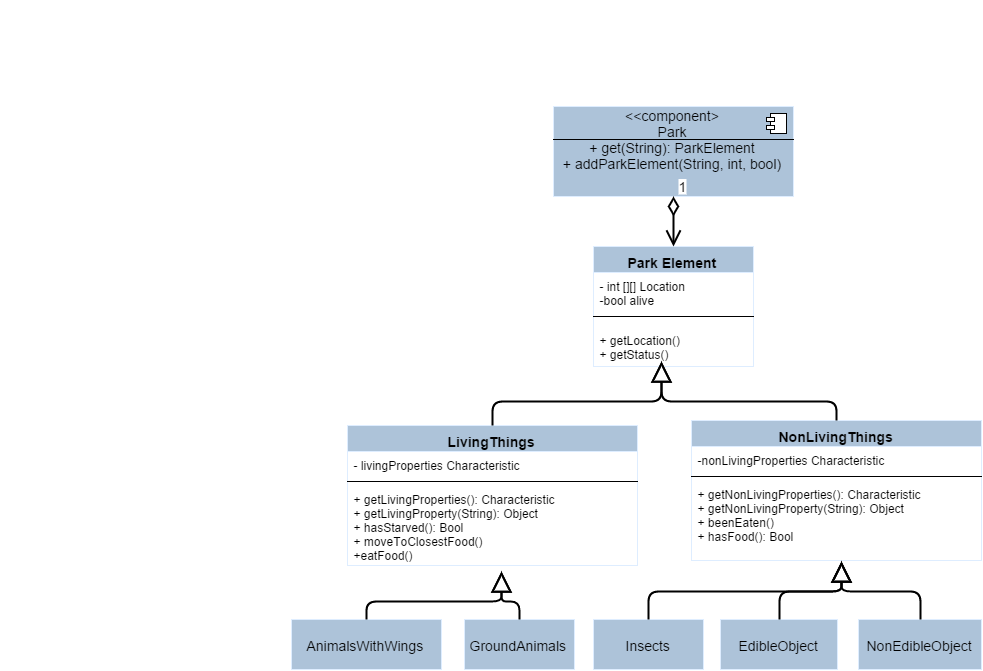
\includegraphics[width=90mm]{ENSE 374 lab diagram.png}
\subsection{Boundary conditions}
When world is created the user shall be allowed to populate the world. If a user inputs far too many items an error shall be received.

 % Stop your text
 \end{document}


